\mbox{$\displaystyle +\,\frac{1}{2}$\,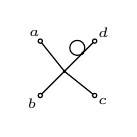
\begin{tikzpicture}[x=0.340cm, y=0.340cm, line width=0.420pt, baseline={([yshift=-0.6ex]0,0)}]
  \draw (-1.016,1.016) -- (-0.113,-0.113);
  \draw (-1.016,-1.016) -- (-0.113,-0.113);
  \draw (1.016,-1.016) -- (-0.113,-0.113);
  \draw (1.016,1.016) -- (0.565,0.565);
  \draw (0.565,0.565) -- (-0.113,-0.113);
  \draw (0.565,0.565) arc[start angle=315.000, end angle=675.000, radius=0.280];
  \fill (0.565,0.565) circle (0.064);
  \fill (-0.113,-0.113) circle (0.064);
  \draw[fill=white] (-1.016,1.016) circle (0.080);
  \draw[fill=white] (-1.016,-1.016) circle (0.080);
  \draw[fill=white] (1.016,-1.016) circle (0.080);
  \draw[fill=white] (1.016,1.016) circle (0.080);
  \node[font=\tiny, inner sep=0pt, anchor=309] at (-1.123,1.149) {$a$};
  \node[font=\tiny, inner sep=0pt, anchor=45] at (-1.137,-1.137) {$b$};
  \node[font=\tiny, inner sep=0pt, anchor=141] at (1.149,-1.123) {$c$};
  \node[font=\tiny, inner sep=0pt, anchor=225] at (1.137,1.137) {$d$};
\end{tikzpicture}}
\diagramgap
\mbox{$\displaystyle +\,\frac{1}{2}$\,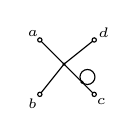
\begin{tikzpicture}[x=0.340cm, y=0.340cm, line width=0.420pt, baseline={([yshift=-0.6ex]0,0)}]
  \draw (-1.016,1.016) -- (-0.113,0.113);
  \draw (-1.016,-1.016) -- (-0.113,0.113);
  \draw (1.016,-1.016) -- (0.565,-0.565);
  \draw (1.016,1.016) -- (-0.113,0.113);
  \draw (0.565,-0.565) -- (-0.113,0.113);
  \draw (0.565,-0.565) arc[start angle=225.000, end angle=585.000, radius=0.280];
  \fill (0.565,-0.565) circle (0.064);
  \fill (-0.113,0.113) circle (0.064);
  \draw[fill=white] (-1.016,1.016) circle (0.080);
  \draw[fill=white] (-1.016,-1.016) circle (0.080);
  \draw[fill=white] (1.016,-1.016) circle (0.080);
  \draw[fill=white] (1.016,1.016) circle (0.080);
  \node[font=\tiny, inner sep=0pt, anchor=315] at (-1.137,1.137) {$a$};
  \node[font=\tiny, inner sep=0pt, anchor=51] at (-1.123,-1.149) {$b$};
  \node[font=\tiny, inner sep=0pt, anchor=135] at (1.137,-1.137) {$c$};
  \node[font=\tiny, inner sep=0pt, anchor=219] at (1.149,1.123) {$d$};
\end{tikzpicture}}
\diagramgap
\mbox{$\displaystyle +\,\frac{1}{2}$\,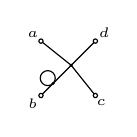
\begin{tikzpicture}[x=0.340cm, y=0.340cm, line width=0.420pt, baseline={([yshift=-0.6ex]0,0)}]
  \draw (-1.016,1.016) -- (0.113,0.113);
  \draw (-1.016,-1.016) -- (-0.565,-0.565);
  \draw (1.016,-1.016) -- (0.113,0.113);
  \draw (1.016,1.016) -- (0.113,0.113);
  \draw (-0.565,-0.565) -- (0.113,0.113);
  \draw (-0.565,-0.565) arc[start angle=315.000, end angle=675.000, radius=0.280];
  \fill (-0.565,-0.565) circle (0.064);
  \fill (0.113,0.113) circle (0.064);
  \draw[fill=white] (-1.016,1.016) circle (0.080);
  \draw[fill=white] (-1.016,-1.016) circle (0.080);
  \draw[fill=white] (1.016,-1.016) circle (0.080);
  \draw[fill=white] (1.016,1.016) circle (0.080);
  \node[font=\tiny, inner sep=0pt, anchor=321] at (-1.149,1.123) {$a$};
  \node[font=\tiny, inner sep=0pt, anchor=45] at (-1.137,-1.137) {$b$};
  \node[font=\tiny, inner sep=0pt, anchor=129] at (1.123,-1.149) {$c$};
  \node[font=\tiny, inner sep=0pt, anchor=225] at (1.137,1.137) {$d$};
\end{tikzpicture}}
\diagramgap
\mbox{$\displaystyle +\,\frac{1}{2}$\,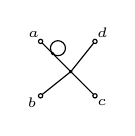
\begin{tikzpicture}[x=0.340cm, y=0.340cm, line width=0.420pt, baseline={([yshift=-0.6ex]0,0)}]
  \draw (-1.016,1.016) -- (-0.565,0.565);
  \draw (-1.016,-1.016) -- (0.113,-0.113);
  \draw (1.016,-1.016) -- (0.113,-0.113);
  \draw (1.016,1.016) -- (0.113,-0.113);
  \draw (-0.565,0.565) -- (0.113,-0.113);
  \draw (-0.565,0.565) arc[start angle=225.000, end angle=585.000, radius=0.280];
  \fill (-0.565,0.565) circle (0.064);
  \fill (0.113,-0.113) circle (0.064);
  \draw[fill=white] (-1.016,1.016) circle (0.080);
  \draw[fill=white] (-1.016,-1.016) circle (0.080);
  \draw[fill=white] (1.016,-1.016) circle (0.080);
  \draw[fill=white] (1.016,1.016) circle (0.080);
  \node[font=\tiny, inner sep=0pt, anchor=315] at (-1.137,1.137) {$a$};
  \node[font=\tiny, inner sep=0pt, anchor=39] at (-1.149,-1.123) {$b$};
  \node[font=\tiny, inner sep=0pt, anchor=135] at (1.137,-1.137) {$c$};
  \node[font=\tiny, inner sep=0pt, anchor=231] at (1.123,1.149) {$d$};
\end{tikzpicture}}
\diagramgap
\mbox{$\displaystyle +\,\frac{1}{2}$\,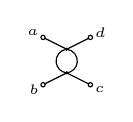
\begin{tikzpicture}[x=0.340cm, y=0.340cm, line width=0.420pt, baseline={([yshift=-0.6ex]0,0)}]
  \draw (-0.884,0.884) -- (0.000,0.442);
  \draw (-0.884,-0.884) -- (0.000,-0.442);
  \draw (0.884,-0.884) -- (0.000,-0.442);
  \draw (0.884,0.884) -- (0.000,0.442);
  \draw (0.000,0.442) arc[start angle=96.026, end angle=263.974, radius=0.444];
  \draw (0.000,0.442) arc[start angle=83.974, end angle=-83.974, radius=0.444];
  \fill (0.000,0.442) circle (0.064);
  \fill (0.000,-0.442) circle (0.064);
  \draw[fill=white] (-0.884,0.884) circle (0.080);
  \draw[fill=white] (-0.884,-0.884) circle (0.080);
  \draw[fill=white] (0.884,-0.884) circle (0.080);
  \draw[fill=white] (0.884,0.884) circle (0.080);
  \node[font=\tiny, inner sep=0pt, anchor=333] at (-1.036,0.960) {$a$};
  \node[font=\tiny, inner sep=0pt, anchor=27] at (-1.036,-0.960) {$b$};
  \node[font=\tiny, inner sep=0pt, anchor=153] at (1.036,-0.960) {$c$};
  \node[font=\tiny, inner sep=0pt, anchor=207] at (1.036,0.960) {$d$};
\end{tikzpicture}}
\diagramgap
\mbox{$\displaystyle +\,\frac{1}{2}$\,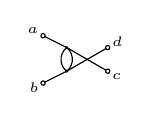
\begin{tikzpicture}[x=0.340cm, y=0.340cm, line width=0.420pt, baseline={([yshift=-0.6ex]0,0)}]
  \draw (-0.884,0.884) -- (0.000,0.442);
  \draw (-0.884,-0.884) -- (0.000,-0.442);
  \draw (1.531,-0.442) -- (0.000,0.442);
  \draw (1.531,0.442) -- (0.000,-0.442);
  \draw (0.000,0.442) arc[start angle=128.594, end angle=231.406, radius=0.565];
  \draw (0.000,0.442) arc[start angle=51.406, end angle=-51.406, radius=0.565];
  \fill (0.000,0.442) circle (0.064);
  \fill (0.000,-0.442) circle (0.064);
  \draw[fill=white] (-0.884,0.884) circle (0.080);
  \draw[fill=white] (-0.884,-0.884) circle (0.080);
  \draw[fill=white] (1.531,-0.442) circle (0.080);
  \draw[fill=white] (1.531,0.442) circle (0.080);
  \node[font=\tiny, inner sep=0pt, anchor=333] at (-1.036,0.960) {$a$};
  \node[font=\tiny, inner sep=0pt, anchor=27] at (-1.036,-0.960) {$b$};
  \node[font=\tiny, inner sep=0pt, anchor=150] at (1.678,-0.527) {$c$};
  \node[font=\tiny, inner sep=0pt, anchor=210] at (1.678,0.527) {$d$};
\end{tikzpicture}}
\diagramgap
\mbox{$\displaystyle +\,\frac{1}{2}$\,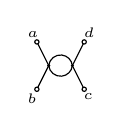
\begin{tikzpicture}[x=0.340cm, y=0.340cm, line width=0.420pt, baseline={([yshift=-0.6ex]0,0)}]
  \draw (-0.884,0.884) -- (-0.442,0.000);
  \draw (-0.884,-0.884) -- (-0.442,0.000);
  \draw (0.884,-0.884) -- (0.442,0.000);
  \draw (0.884,0.884) -- (0.442,0.000);
  \draw (-0.442,0.000) arc[start angle=186.026, end angle=353.974, radius=0.444];
  \draw (-0.442,0.000) arc[start angle=173.974, end angle=6.026, radius=0.444];
  \fill (-0.442,0.000) circle (0.064);
  \fill (0.442,0.000) circle (0.064);
  \draw[fill=white] (-0.884,0.884) circle (0.080);
  \draw[fill=white] (-0.884,-0.884) circle (0.080);
  \draw[fill=white] (0.884,-0.884) circle (0.080);
  \draw[fill=white] (0.884,0.884) circle (0.080);
  \node[font=\tiny, inner sep=0pt, anchor=297] at (-0.960,1.036) {$a$};
  \node[font=\tiny, inner sep=0pt, anchor=63] at (-0.960,-1.036) {$b$};
  \node[font=\tiny, inner sep=0pt, anchor=117] at (0.960,-1.036) {$c$};
  \node[font=\tiny, inner sep=0pt, anchor=243] at (0.960,1.036) {$d$};
\end{tikzpicture}}
